\part{Berechenbarkeit}

\paragraph*{Uns interessieren Fragestellungen der Art} Was kann man überhaupt berechnen? Was sind geeignete Rechenmodelle?

\paragraph*{Notation} endliches Alphabet $\Sigma i$ oft: $\Sigma = \{ 0,1 \}$ Die Menge aller Wörter der Länge $k$ über $\Sigma$ bezeichnen wir als $\sum\limits^k$, z.B. \note{kanonische oder lexikographisch Reihenfolge} $$ \{ 0,1 \}^3 = \{ 000,001,010,011,100,101,110,111 \} $$

\paragraph*{Probleme} $\overset{\wedge}{=}$ 'Aufgaben' oder 'Fragestellungen', die wir mit dem Rechner lösen/beantworten wollen.


\subsection*{Problem 1.1}
\paragraph*{Eingabe} eine binär kodierte Zahl $q \in \mathbb{N}$; $q \geq 2$

\paragraph*{Ausgabe} ein binär kodierter Primfaktor von $q$

\paragraph*{Bsp.} Eingabe: 110 (die Zahl 6); Ausgabe: 010 (die Zahl 2) oder 011 (die Zahl 3)

\note{bin() Binärkodierung}\note{$\{ 0,1 \}^*$ endliches Wort}
\par\medskip
Das Problem samt Lösungen entspricht der Relation $R \subseteq \{ 0,1 \}^* \times \{ 0,1 \}$ mit $R=\{ (x,y) \in \{ 0,1 \}^* \times \{ 0,1 \}^* \| x=bin(q), y=bin(q); p,q \in \mathbb{N}, q \geq 2, p$ prim, $p$ teilt $q \}$. Relation, da für gegebene Eingabe mehrere Ergebnisse möglich sind.
\par\medskip

\subsection*{Problem 1.2 (Multiplikation)}
\paragraph*{Eingabe} zwei binär kodierte Zahlen $a,b \in \mathbb{N}$.
\paragraph*{Ausgabe} binär kodierte Zahl $c \in \mathbb{N}$ mit $c=a \cdot b$.

\par\medskip
Um die Zahl $a$ und $b$ in der Eingabe unterscheiden zu können, führen wir ein Trennsymbol ein, also $\Sigma = \{ 0,1,\# \}$. Die kodierte Eingabe ist dann $bin(a)\#bin(b)$ die kodierte Ausgabe ist $f(bin(a)\#bin(b))=bin(c)$
\par\bigskip
Wir werden uns im folgenden meistens mit Ja/Nein-Fragen beschäftigen, sogenannte Entscheidungsprobleme. Diese haben die Form $$ f:\Sigma^* \rightarrow \{ 0,1 \} $$ wobei wir '0' als NEIN interpretieren und '1' als JA. $ L=f^{-1}(1) \subseteq \sum^* $ ist die Menge der Eingaben, die mit 1 beantwortet werden. $L$ nennen wir auch eine Sprache.
\par\medskip

\subsection*{Problem 1.3 (Graphzusammenhang)}
\paragraph*{Eingabe} Kodierung eines Graphen $G(V,E)$ (gerichtet).
\paragraph*{Ausgabe} Das Zeichen 1, falls $G$ zusammenhängend, sonst 0.

\par\medskip Graphen könnte man kodieren als $$ \underbrace{bin(n)}_{\# Knoten = |V|}\# \underbrace{010 \dots}_{\substack{|V| \cdot |V| \text{ bits entsprechend} \\ \text{der Adjazenzmatrix von } G} } $$

$$ \begin{pmatrix}
1 & 2 & \cdot \\
2 & \cdot & \cdot \\
\cdot & \cdot & i-n,j-n
\end{pmatrix} $$

\par\medskip Es sind natürlich nicht alle Wörter über $\Sigma^*$ eine gültige Kodierung eines Graphen. Sei $\mathcal{G}$ die Menge aller Graphen, $\mathcal{G}_z \subseteq \mathcal{G}$ die Menge aller zusammenhängenden Graphen, und $code(G)$ für $G \in \mathcal{G}$ die Kodierung eines Graphen. Dann ist die entsprechende Sprache $$ L=\{ w \in \{ 0,1,\# \}^* \| \exists G(V,E) \in \mathcal{G}_z, w=code(G) \} $$ Die Sprache $L$ enthält alle Eingaben, die einen zusammenhängenden Graphen kodieren.

\par\medskip Das Komplement von $L$ ist definiert als $$ \overline{L} := \Sigma^* \textbackslash L $$ $\overline{L}$ enthält Eingaben, die keiner korrekten Kodierung eines Graphen entsprechen oder Graphen, welche nicht zusammenhängend sind.


\section{Rechnermodelle}

\subsection{Turingmaschine (TM)}
Eine Turingmaschine arbeitet auf einem beidseitig unendlichen Speicherband,

\begin{center}
\begin{tikzpicture}[start chain=1 going right,start chain=2 going below,node distance=-0.15mm]
    \node [on chain=2] {Band};
    \node [on chain=1] at (-1.5,-.4) {\ldots};  
    \foreach \x in {1,2,...,11} {
        \x, \node [draw,on chain=1] {};
    } 
    \node [name=r,on chain=1] {\ldots}; 
    \node [name=k, arrow box, draw,on chain=2,
        arrow box arrows={east:.25cm, west:0.25cm}] at (-0.335,-.65) {};    
    \node at (1,-.85) {LS-Kopf};
    \node [on chain=2] {};
\end{tikzpicture}
\end{center}

welches aus Zellen besteht. Jede Zelle enthält ein Element des sogenannten Bandalphabets $\Gamma$, z.B. $\Gamma=\{ 0,1,B \}$. Des Weiteren hat eine Turingmaschine einen Schreib-/Lesekopf, der über das Band wandern kann und jeweils den Inhalt der Zelle, über der er steht, lesen und schreiben kann. Daneben besitzt eine Turingmaschine auch noch einen Zustand $q \in Q$ aus einer endlichen Zustandsmenge $Q$.

\par\medskip Per Konvention befindet sich die Turingmaschine am Anfang einer Rechnung im Anfangszustand $q_0 \in Q$, auf dem Band steht (startend mit der Zelle, auf die der Schreib-/Lesekopf zeigt) von links nach rechts die Eingabe, alle anderen Zellen enthalten das Leerzeichen ($B$).

\par\medskip Das Eingabealphabet $\Sigma \subseteq \Gamma \backslash \{B\}$. Die Arbeitsweise der Turingmaschine wird durch eine Übergangsrelation: $$ \delta : (Q \backslash \{ \overline{q}\} \times \Gamma \times Q \times \Delta \times \{ R,L,N \}) $$ ausgedrückt. Hierbei ist $\overline{q} \in Q$ ein besonderer Zustand, der stopp-Zustand.

\par\medskip
\begin{itemize}
	\item[] $Q \backslash \{ \overline{q}\}$: Zustand
	\item[] $\Gamma$: gelesenes Zeichen / zu schreibendes Zeichen
	\item[] $Q$: neuer Zustand
	\item[] $\{ R,L,N \}$: Kopfbewegung
\end{itemize}

\par\medskip Falls für gegebenen Zustand und Zeichen unter dem Schreib-/Lesekopf nur eine Aktion möglich ist, reden wir von einer Übergangsfunktion. $$ \delta : (Q \backslash \{ \overline{q}\}) \times \Gamma \rightarrow Q \times \Gamma \times \{R,L,N\} $$ $\delta(q,a)=(q',a',d)$ bedeutet: wenn die Turingmaschine im Zustand $q$ ist und Zeichen $a$ ließt, schreibe Zeichen $a'$ an diese Stelle, bewege Kopf nach $d \in \{L,R,N\}$ und nimm Zustand $q'$ ein.

\par\medskip Eine Turingmaschine führt so lange Rechenschritte aus, bis der stopp-Zustand $\overline{q}$ erreicht wird.

\paragraph*{Bsp.} Übergangsfunktion $\delta$
\begin{center}
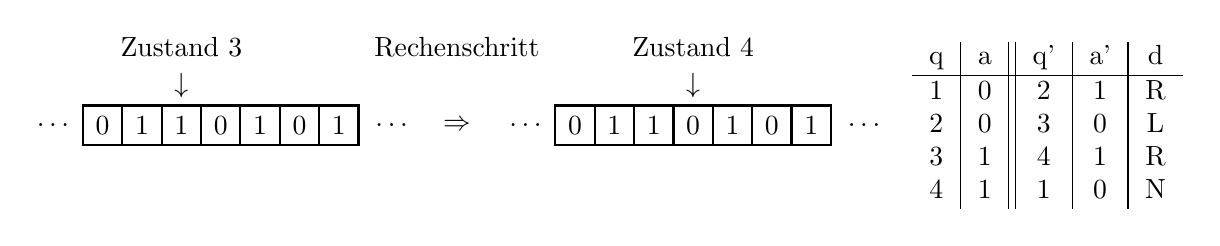
\begin{tikzpicture}

	% Band 1
	\node at (-0.1,0) {\dots};
	\node (rect) at (0.5,0) [draw,thick,minimum width=0.5cm,minimum height=0.5cm] {0};
	\node (rect) at (1,0) [draw,thick,minimum width=0.5cm,minimum height=0.5cm] {1};
	\node (rect) at (1.5,0) [draw,thick,minimum width=0.5cm,minimum height=0.5cm] {1};
	\node (rect) at (2,0) [draw,thick,minimum width=0.5cm,minimum height=0.5cm] {0};
	\node (rect) at (2.5,0) [draw,thick,minimum width=0.5cm,minimum height=0.5cm] {1};
	\node (rect) at (3,0) [draw,thick,minimum width=0.5cm,minimum height=0.5cm] {0};
	\node (rect) at (3.5,0) [draw,thick,minimum width=0.5cm,minimum height=0.5cm] {1};
	\node at (4.2,0) {\dots};
	
	\node at (5,1) {Rechenschritt};
	\node at (5,0) {$\Rightarrow$};
	
	% Band 2
	\node at (5.9,0) {\dots};
	\node (rect) at (6.5,0) [draw,thick,minimum width=0.5cm,minimum height=0.5cm] {0};
	\node (rect) at (7,0) [draw,thick,minimum width=0.5cm,minimum height=0.5cm] {1};
	\node (rect) at (7.5,0) [draw,thick,minimum width=0.5cm,minimum height=0.5cm] {1};
	\node (rect) at (8,0) [draw,thick,minimum width=0.5cm,minimum height=0.5cm] {0};
	\node (rect) at (8.5,0) [draw,thick,minimum width=0.5cm,minimum height=0.5cm] {1};
	\node (rect) at (9,0) [draw,thick,minimum width=0.5cm,minimum height=0.5cm] {0};
	\node (rect) at (9.5,0) [draw,thick,minimum width=0.5cm,minimum height=0.5cm] {1};
	\node at (10.2,0) {\dots};
	
	% Zustand tag
	\node at (1.5,1) {Zustand 3};
	\node at (1.5,0.5) {$\downarrow$};
	
	\node at (8,1) {Zustand 4};
	\node at (8,0.5) {$\downarrow$};
	
	\node at (12.5,0) {
	\begin{tabular}{c|c||c|c|c}
		q & a & q' & a' & d \\
		\hline
		1 & 0 & 2 & 1 & R \\
		2 & 0 & 3 & 0 & L \\
		3 & 1 & 4 & 1 & R \\
		4 & 1 & 1 & 0 & N \\
		\end{tabular}
	};
	
\end{tikzpicture}
\end{center}

\paragraph*{Zusammenfassung} Eine Turingmaschine wird definiert durch
\begin{itemize}
	\item endliche Zustandsmenge $Q$
	\item endliches Eingabealphabet $\Sigma \supseteq \{ 0,1 \}$
	\item endliches Bandalphabet $\Gamma \supset \Sigma$
	\item $B \in \Gamma\backslash\Sigma$ (Leerzeichen)
	\item $q_0 \in Q$ (Anfangszeichen)
	\item $\overline{q} \in Q$ (stopp-Zustand)
	\item Übergangsfunktion $\delta : (Q \backslash \{ \overline{q} \}) \times \Gamma \rightarrow Q \times \Gamma \times \{ R,L,N \}$
\end{itemize}

\par\medskip Eine Turingmaschine ist also durch ein 7-Tupel ($Q,\Sigma,\Gamma,B,q_0,\overline{q},\delta$) definiert. Eine Konfiguration einer Turingmaschine ist ein Schnappschuss der Rechnung, zu einem bestimmten Zeitpunkt und beschreibt vollständig alle Details, die notwendig sind, um die Rechnung fortzusetzen, d.h. Bandinhalt, Zustand, Kopfposition.\par

\medskip Formel:
\begin{itemize}
	\item Konfiguration ist ein String $\alpha q \beta$ mit $q \in Q$, $\alpha,\beta \in \gamma^*$ welche bedeutet, dass auf Band $\alpha\beta$ steht (eingerahmt von Blanks), Zustand $q$ ist und LS-Kopf auf erstem Zeichen von $B$ steht.
	\item $\alpha'q'\beta'$, ist direkte Nachfolgekonfiguration $\alpha q \beta$, falls $\alpha'q'\beta'$ in einem Rechenschritt aus $\alpha q \beta$ entsteht, wir schreiben $\alpha q \beta \vdash \alpha'q'\beta'$.
	\item $\alpha''q''\beta''$ ist Nachfolgekonfiguration von $\alpha'q'\beta'$, falls $\alpha''q''\beta''$ in endlich vielen Rechenschritten aus $\alpha q \beta$ entspricht. Wir schreiben $\alpha q \beta \vdash^* \alpha''q''\beta''$.
\end{itemize}

\par\medskip Die Rechnung terminiert sobald der stopp-Zustand $\overline{q}$ erreicht ist. Dann gibt es keine Nachfolgekonfiguration. Die Laufzeit einer TM-Rechnung ist Zahl der Rechenschritte, die Turingmaschine bis zur Terminierung ausführt. Falls die Rechnung nicht terminiert, ist Laufzeit unbeschränkt. Der Platzverbrauch einer TM-Rechnung ist die Anzahl besuchter Bandzellen (kann auch unbeschränkt sein).


\section{TM-berechenbare Funktionen und Sprachen}

Eine Turingmaschine $M$, die für jede Eingabe terminiert, berechnet eine totale Funktion $$f_M:\sum\limits^* \rightarrow \sum\limits^*$$ Wenn der stopp-Zustand $\overline{q}$ erreicht ist, kann das Ergebnis $f_M(x)$ rechts vom LS-Kopf vom Band gelesen werden (bis zum ersten Zeichen nicht in $\Sigma$). Das Ergebnis kann auch $\varepsilon$ sein, \note{$\varepsilon$ Das leere Wort} falls LS-Kopf nach Beendung auf einem Zeichen nicht aus $\Sigma$ ist. Manche Turingmaschinen terminieren nicht, wir erweitern deshalb die Funktion $f_M$ wie folgt: $$ f_M:\sum\limits^* \rightarrow \sum\limits^* \cup \{ \perp \} $$ $'\perp'$ (Bottom) steht für 'nicht definiert', d.h. wenn $M$ auf die Eingabe nicht terminiert.